\titleformat {\chapter} {\normalfont\huge\bfseries\color{black}}   {\thechapter}{10pt}{\huge} 
\chapter {Simulation Results}

%% ================================
%% \input{Advice-on-Chapter-4}
%% ================================
	
\section{The Parametric Equations}
%% \label{sec:4.1-CNC-Research-Machine}

The ten(10) 2D parametric curves covered in this work are:
\begin{enumerate}
	\item Teardrop
	\item Butterfly
	\item Ellipse
	\item Skewed-Astroid
	\item Circle
	\item AstEpi = Astroid + Epicycloid combination
	\item Snailshell
	\item SnaHyp = Snailshell + Hypotrocoid combination
	\item Ribbon-10L
	\item Ribbon-100l = 10 times scaleup of Ribbon-10L
	
\end{enumerate}

The parametric equations describing each of the curves x(u), and y(u) are provided in the next table. The independent parameter u is limited to
\begin{equation}
u  \in  [0.0, 1.0] \nonumber
\end{equation}

The curves were selected based on their different characteristics like closed loop curves, open ended curves, symmetric or non-symmetric about the x-axis and y-axis, and having concave or convex turns. The x and y dimensions (sizes) vary among the different curves. \vspace*{1\baselineskip}

The main objective of the selection criteria is to ensure that the interpolation algorithm for the parametric curve succeeds and does not break in all cases. \vspace*{1\baselineskip}
	
The results for the feedrates in machining the ten(10) curves show continuity, smoothness, with no abrupt jumps as the CNC machine traverse the entire curve from the start (u = 0.0) until the end (u = 1.0).	\vspace*{1\baselineskip}
		
%% \pagebreak

%% ================================================

%% \pagebreak

%% ================================================

%% \pagebreak

%% ================================================

%% \pagebreak

%% ================================================

%% \pagebreak

%% ================================================

\pagebreak

%% ===================================================================
%% \section{Feedrate Plot Profiles}




\pagebreak

%% ===================================================================
%% \section{Algorithm Run Data Summaries} 


%% ===================================================================
\pagebreak
%% \subsection{Teardrop and Butterfly}

\begin{figure}[htbp]
\begin{center}
	\frame{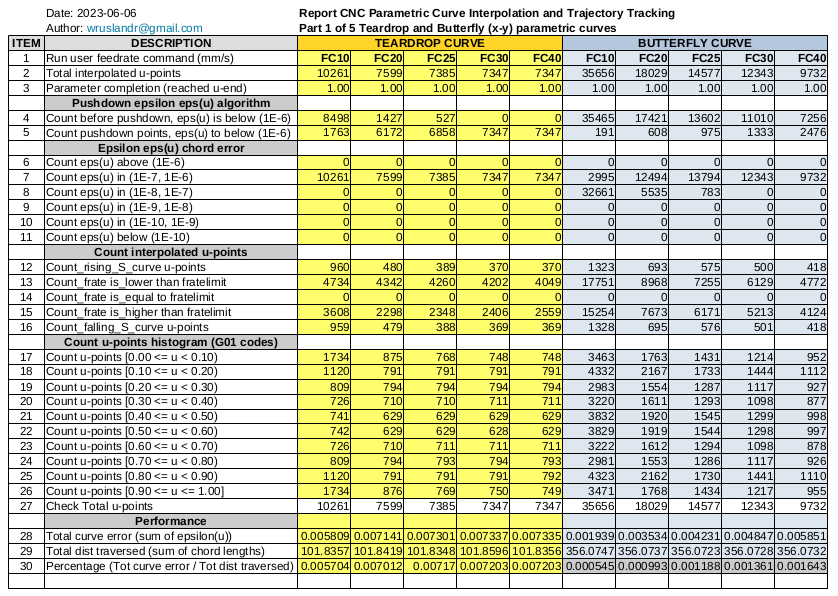
\includegraphics[width=1.00\textwidth]{./07-images/img-Ch52/Teardrop-and-Butterfly-run-data-summary.png}}\\
	\frame{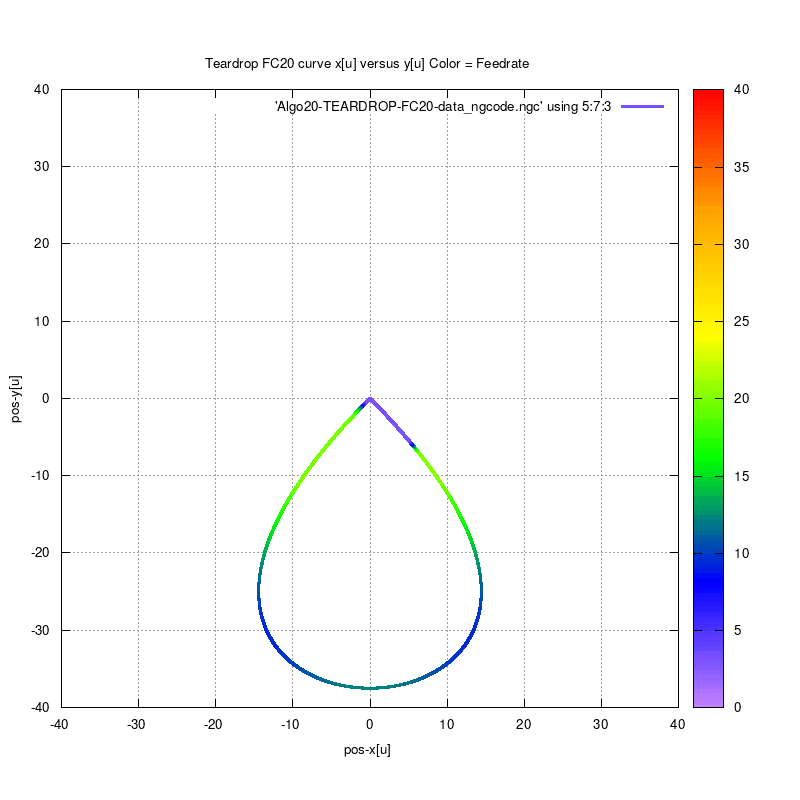
\includegraphics[width=0.49\textwidth]{./07-images/img-Ch5/TEARDROP-Feedrate.png}}
	\frame{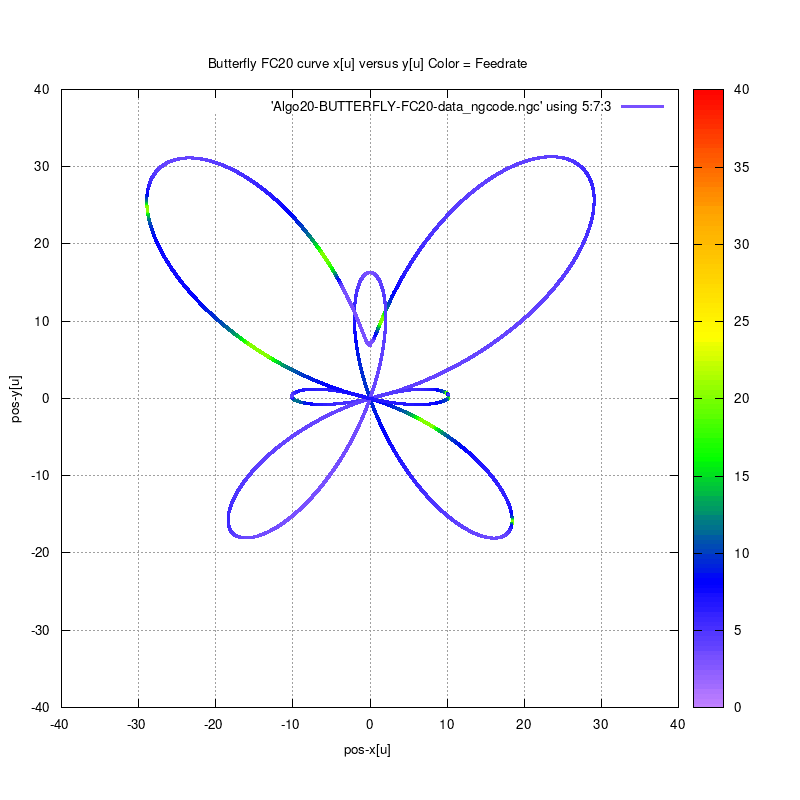
\includegraphics[width=0.49\textwidth]{./07-images/img-Ch5/BUTTERFLY-Feedrate.png}}\\
	\caption{Teardrop and Butterfly run data summary}
	\label{fig:Teardrop and Butterfly run data summary.png}
\end{center}
\end{figure}


%% ===================================================================
\pagebreak
%% \subsection{Ellipse and Skewed-Astroid}
\begin{figure}[htbp]
	\begin{center}
		\frame{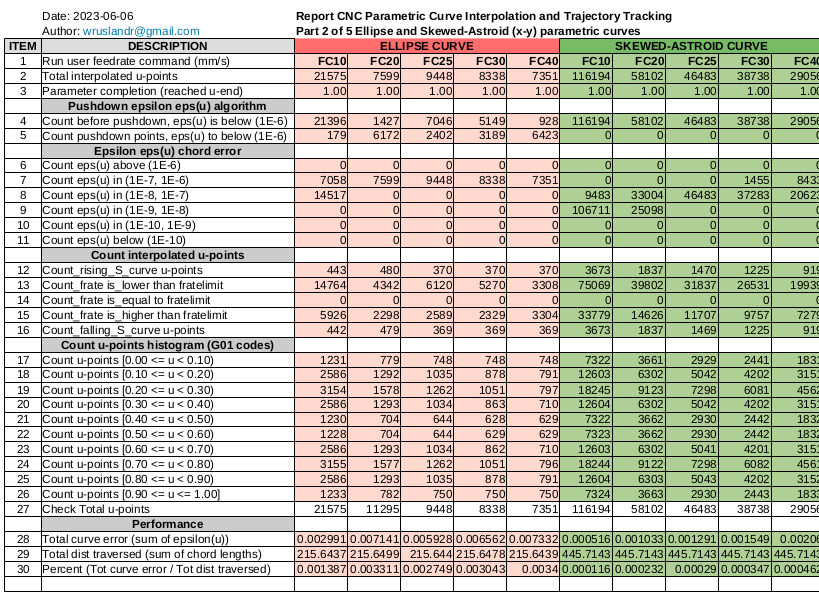
\includegraphics[width=1.00\textwidth]{./07-images/img-Ch52/Ellipse-and-Skewed-Astroid-run-data-summary.png}}\\
		\frame{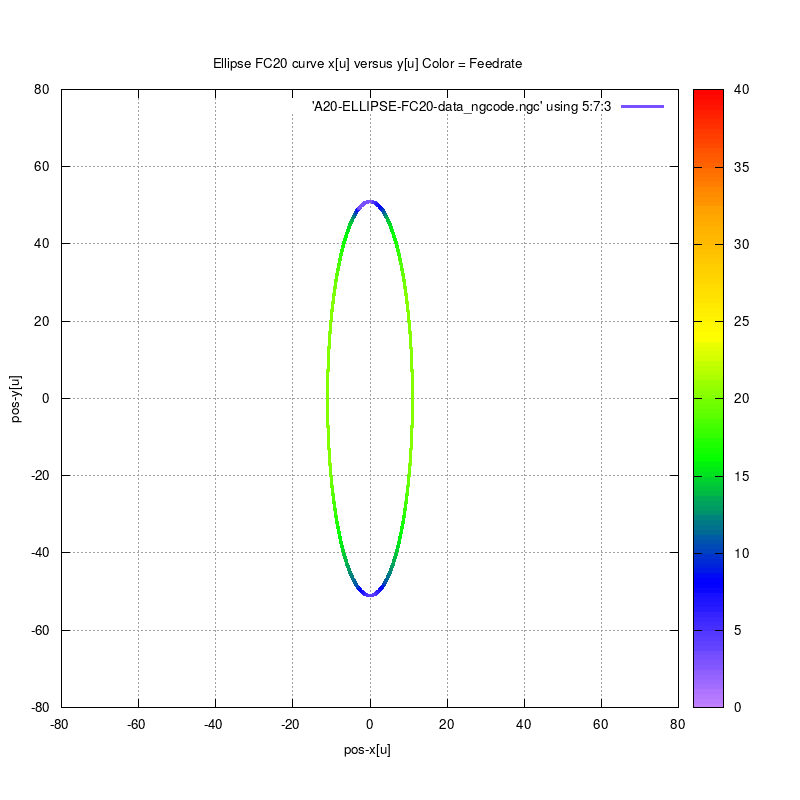
\includegraphics[width=0.49\textwidth]{./07-images/img-Ch5/ELLIPSE-Feedrate.png}}
		\frame{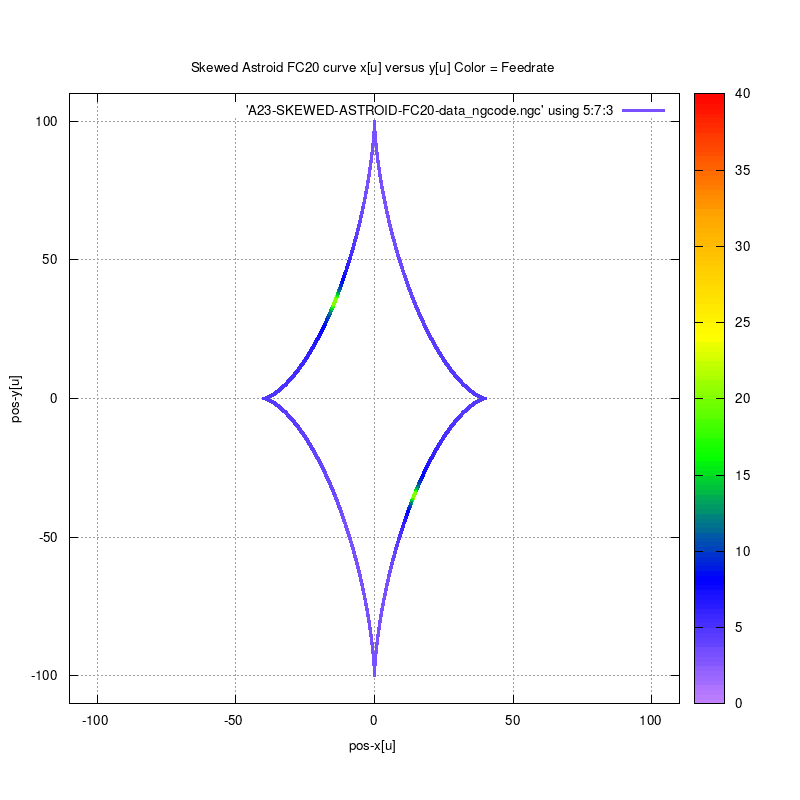
\includegraphics[width=0.49\textwidth]{./07-images/img-Ch5/SKEWED-ASTROID-Feedrate.png}}\\

		\caption{Ellipse and Skewed-Astroid run data summary}
		\label{fig:Ellipse and Skewed-Astroid run data summary.png}
	\end{center}
\end{figure}

%% ===================================================================
\pagebreak
%% \subsection{Circle and AstEpi}
\begin{figure}[htbp]
	\begin{center}
		\frame{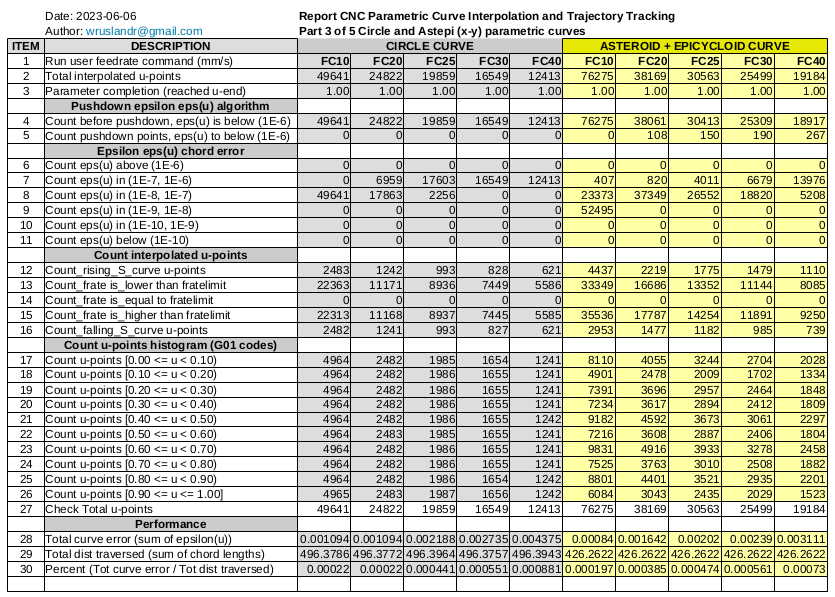
\includegraphics[width=1.00\textwidth]{./07-images/img-Ch52/Circle-and-AstEpi-run-data-summary.png}}\\
		\frame{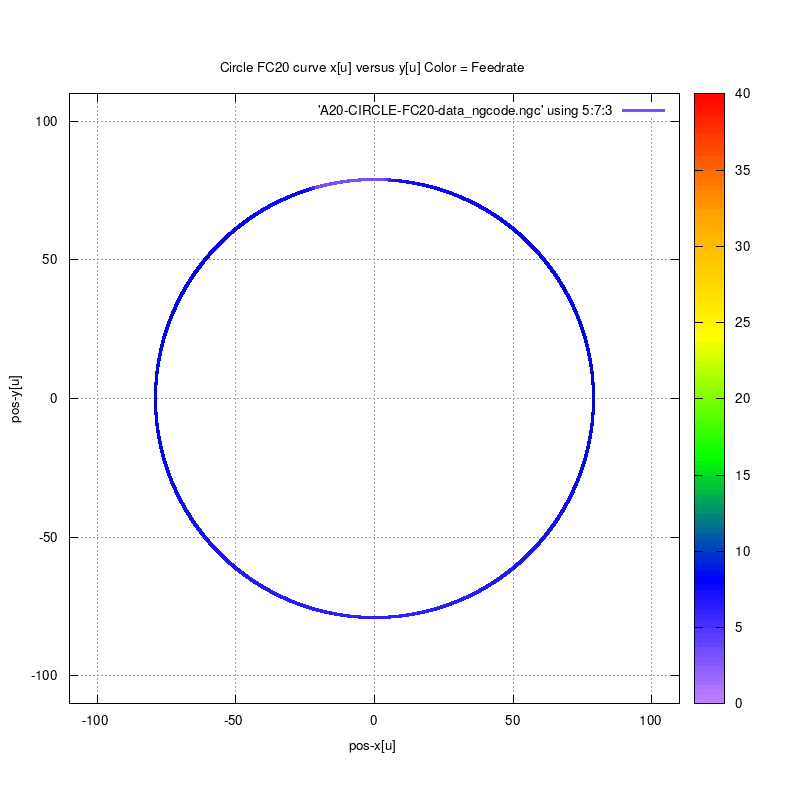
\includegraphics[width=0.49\textwidth]{./07-images/img-Ch5/CIRCLE-Feedrate.png}}
        \frame{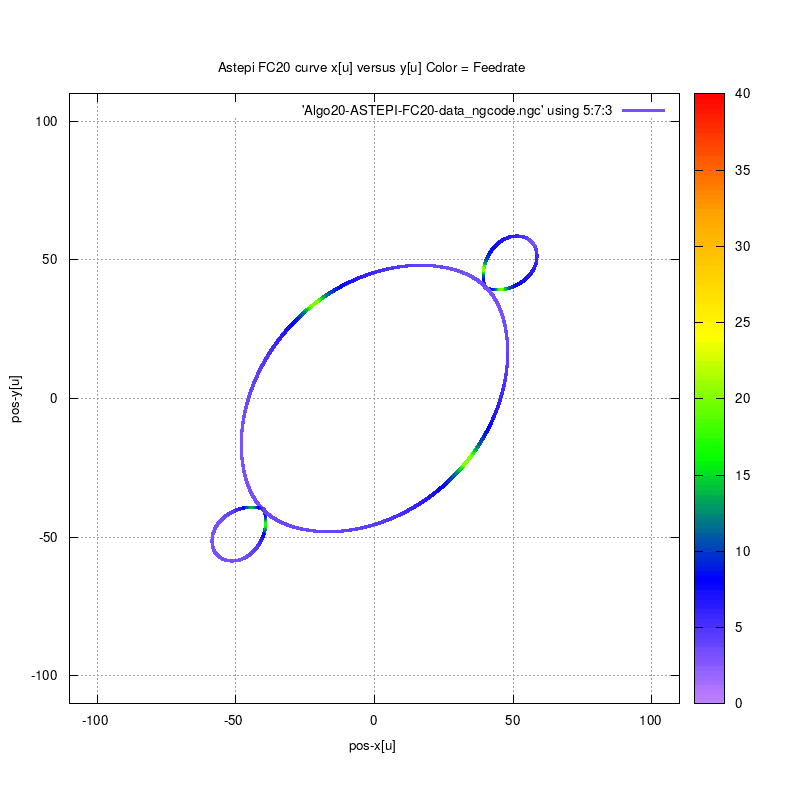
\includegraphics[width=0.49\textwidth]{./07-images/img-Ch5/ASTEPI-Feedrate.png}}\\
		
		\caption{Circle and AstEpi run data summary}
		\label{fig:Circle and AstEpi run data summary.png}
	\end{center}
\end{figure}

\pagebreak
%% \subsection{Snailshell and SnaHyp}
\begin{figure}[htbp]
	\begin{center}
		\frame{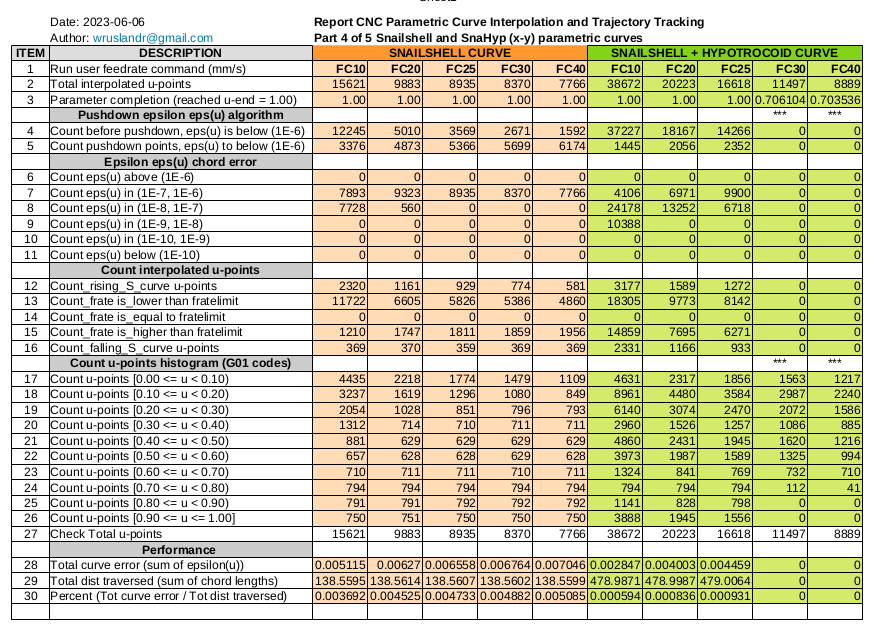
\includegraphics[width=1.00\textwidth]{./07-images/img-Ch52/Snailshell-and-SnaHyp-run-data-summary.png}}\\
		\frame{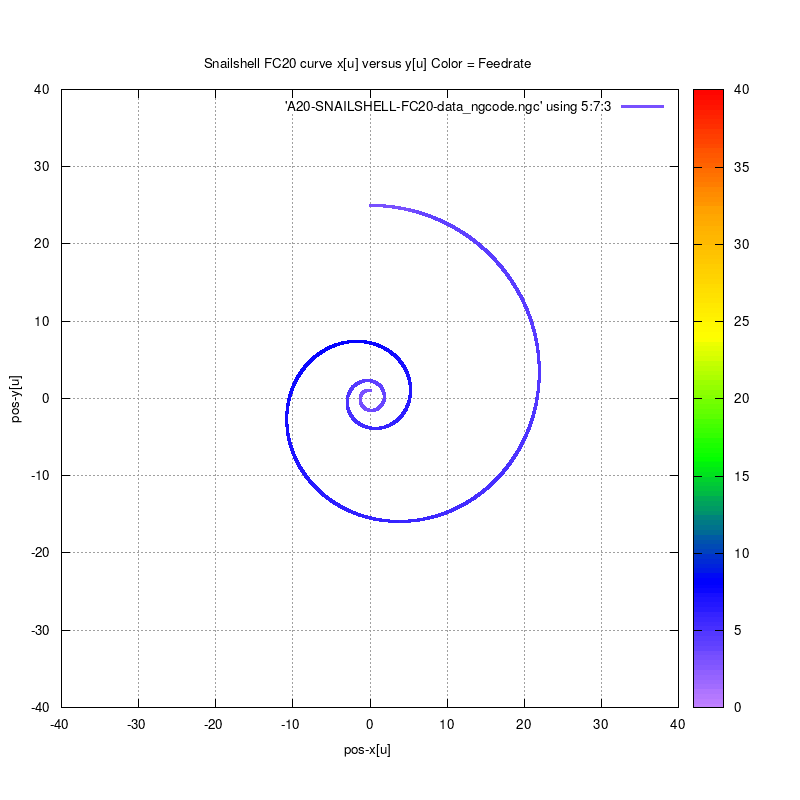
\includegraphics[width=0.49\textwidth]{./07-images/img-Ch5/SNAILSHELL-Feedrate.png}}
        \frame{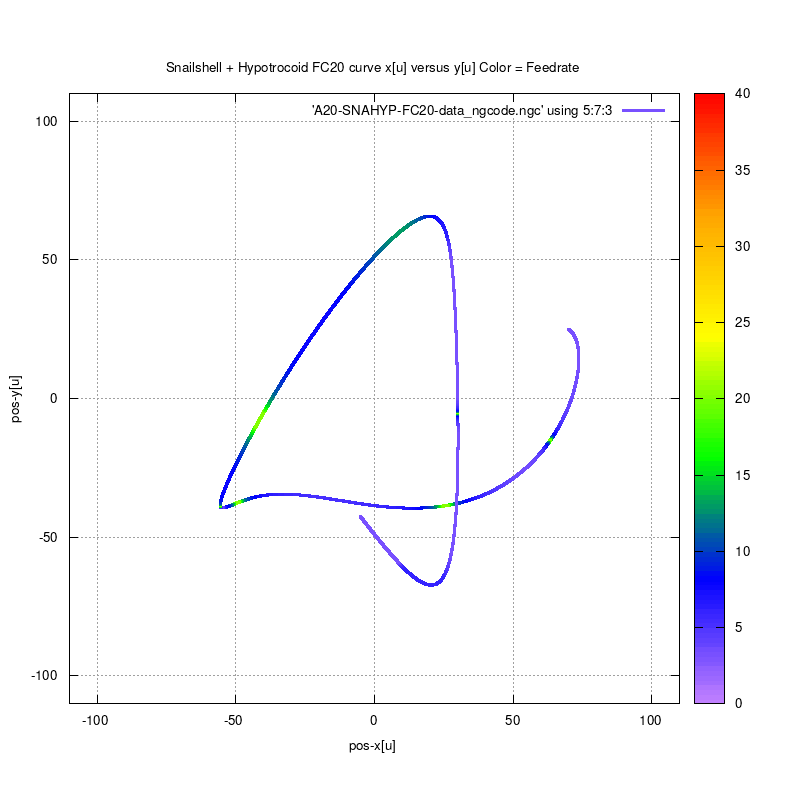
\includegraphics[width=0.49\textwidth]{./07-images/img-Ch5/SNAHYP-Feedrate.png}}\\

		\caption{Snailshell and SnaHyp run data summary}
		\label{fig:Snailshell and SnaHyp run data summary.png}
	\end{center}
\end{figure}



%% ===================================================================
\pagebreak
%% \subsection{Ribbon-10L and Ribbon-100L}
\begin{figure}[htbp]
	\begin{center}
		\frame{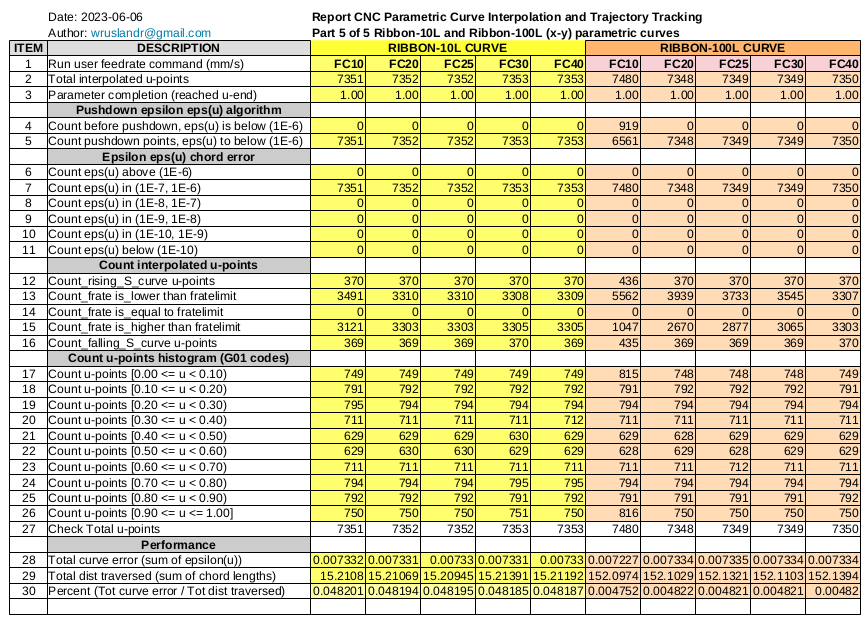
\includegraphics[width=1.00\textwidth]{./07-images/img-Ch52/Ribbon-10L-and-Ribbon-100L-run-data-summary.png}}\\
		\frame{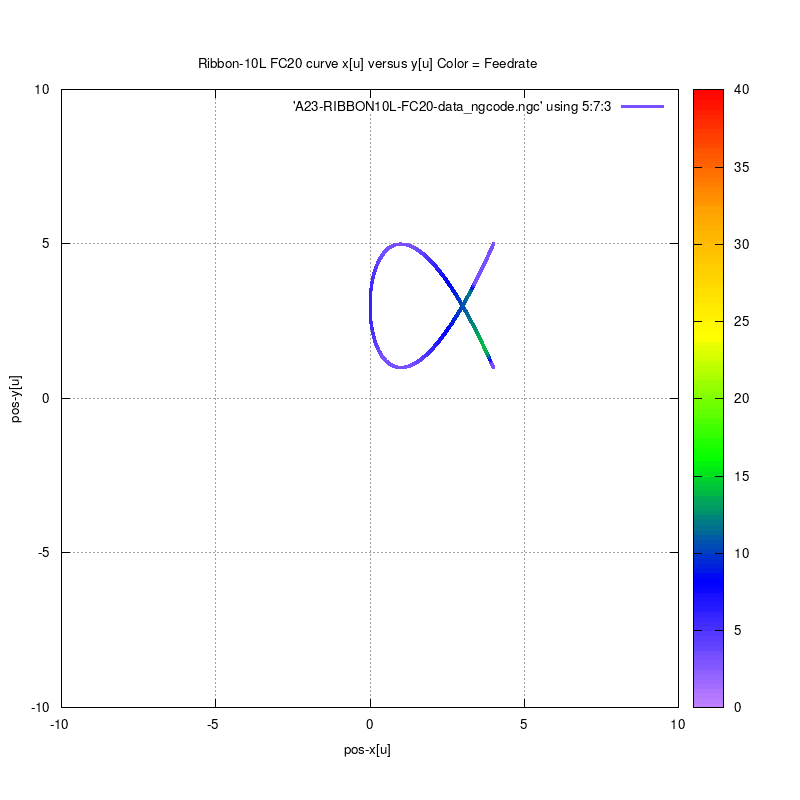
\includegraphics[width=0.49\textwidth]{./07-images/img-Ch5/RIBBON-10L-Feedrate.png}}
        \frame{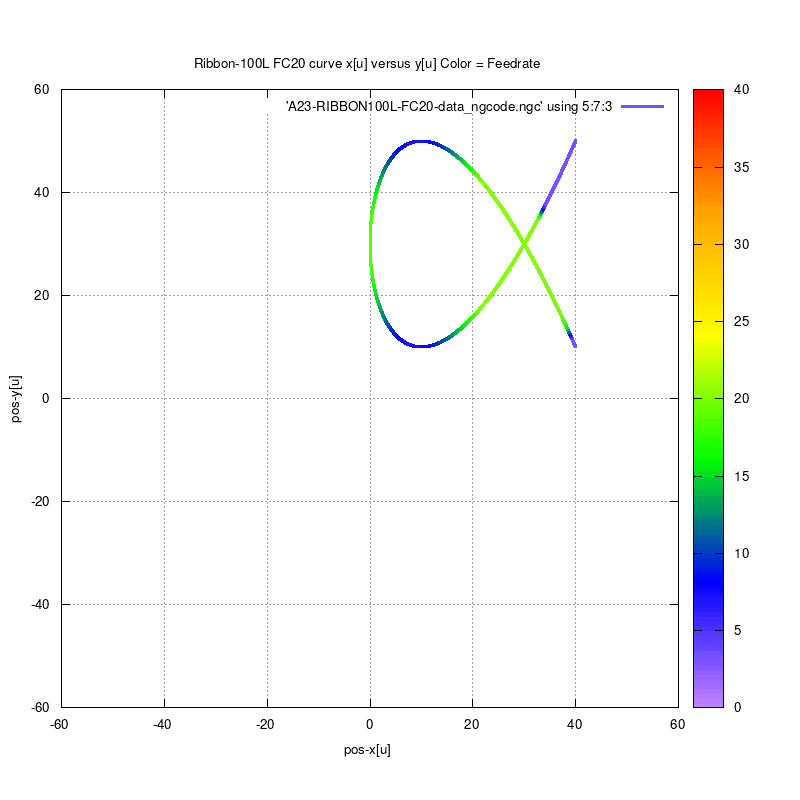
\includegraphics[width=0.49\textwidth]{./07-images/img-Ch5/RIBBON-100L-Feedrate.png}}\\

		\caption{Ribbon-10L and Ribbon-100L run data summary}
		\label{fig:Ribbon-10L and Ribbon-100L run data summary.png}
	\end{center}
\end{figure}


\pagebreak
%% =============================================================

%% \section{Run Feedrate Profiles}











%%
%% \begin{figure}[htbp]
%% \begin{center}
%%	\frame{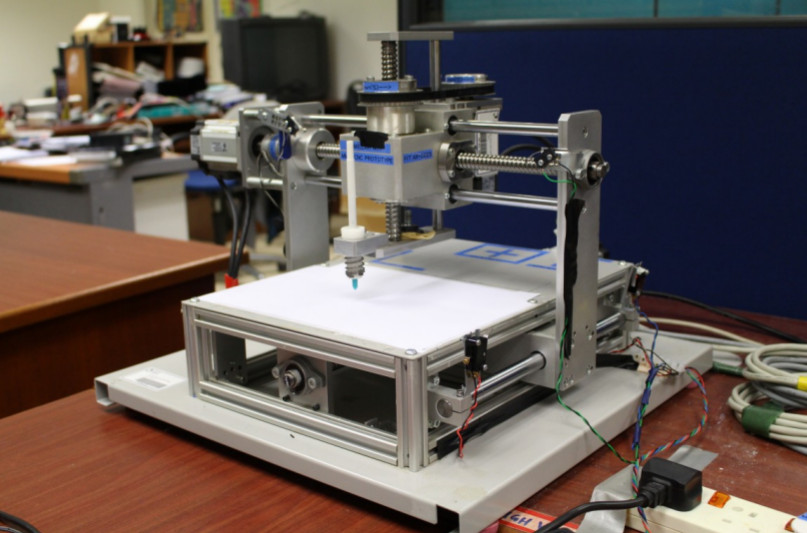
\includegraphics[width=0.85\textwidth]{./07-images/img-Ch4/CNC-Research-Machine-3-Axis.jpg}}
%%	\caption{The UMP 3-axis CNC Research Machine}
%%	\label{fig:CNC-Research-Machine-3-Axis.jpg}
%% \end{center}
%% \end{figure}



% ================== END CHAPTER-5 ========================